\section{Consistency and Limiting Distributions}

\subsection{Convergence in Probability}

In this section, we formalize the notion of a sequence of random variables $\{X_n\}$ getting "close" to another random variable $X$ as $n \to \infty$. We say $X_n$ \textbf{converges in probability} to $X$, denoted as $X_n \overset{P}{\to} X$, if $P(|X_n - X| \geq \epsilon) \to 0$ for all $\epsilon > 0$.

One way to demonstrate convergence in probability is to use Chebyshev's Theorem: for a random variable $X$ with variance $\sigma^2 < \infty$, and for any $k > 0$, we have $P(|X - \mu| \geq k\sigma) \leq \frac{1}{k^2}$.

Let $\{X_n\}$ be a sequence of independent and identically distributed (i.i.d.) random variables with mean $\mu$ and variance $\sigma^2 < \infty$. Let $\overline{X}_n = \frac{1}{n} \sum_{i=1}^n X_i$. Then $\overline{X}_n \overset{P}{\to} \mu$.

\begin{proof}
The mean and variance of $\overline{X}_n$ are $\mu$ and $\frac{\sigma^2}{n}$, respectively. By Chebyshev's Theorem, for all $\epsilon > 0$, we have
\[
P(|\overline{X}_n - \mu| \geq \epsilon) = P\left(|\overline{X}_n - \mu| \geq \frac{\epsilon \sqrt{n}}{\sigma} \cdot \frac{\sigma}{\sqrt{n}}\right) \leq \frac{\sigma^2}{n\epsilon^2} \to 0.
\]
\end{proof}

The Weak Law of Large Numbers (WLLN) implies that all the mass of the distribution of $\overline{X}_n$ converges to $\mu$. In a sense, for large $n$, $\overline{X}_n$ is close to $\mu$. But how close is it? For example, if we were to estimate $\mu$ by $\overline{X}_n$, what can we say about the error of estimation? Actually, a Strong Law of Large Numbers (SLLN) can be proved. Moreover, we can weaken the hypothesis of the WLLN to require only that the $X_i$ are i.i.d. with finite mean $\mu$. Thus, the SLLN is a first moment theorem, while the WLLN requires the existence of the second moment.

Next, we list several theorems concerning convergence in probability, which is closed under linearity.

\begin{theorem}
Suppose $X_n \overset{P}{\to} X$ and $Y_n \overset{P}{\to} Y$. Then $X_n + Y_n \overset{P}{\to} X + Y$.
\end{theorem}
\begin{proof}
Using the triangle inequality, we have
\[
P(|(X_n + Y_n) - (X + Y)| \geq \epsilon) \leq P(|X_n - X| + |Y_n - Y| \geq \epsilon) \leq P\left(|X_n - X| \geq \frac{\epsilon}{2}\right) + P\left(|Y_n - Y| \geq \frac{\epsilon}{2}\right).
\]
\end{proof}

\begin{theorem}
For any constant $a$, if $X_n \overset{P}{\to} X$, then $aX_n \overset{P}{\to} aX$.
\end{theorem}
\begin{theorem}
If $X_n \overset{P}{\to} a$ and the real function $g$ is continuous at $a$, then $g(X_n) \overset{P}{\to} g(a)$.
\end{theorem}
\begin{proof}
Since $g$ is continuous at $a$, for all $\epsilon > 0$, there exists $\delta > 0$ such that $|g(x) - g(a)| < \epsilon$ for $|x - a| < \delta$. Thus, $|g(x) - g(a)| \geq \epsilon$ implies $|x - a| \geq \delta$. Substituting $X_n$ for $x$, we obtain
\[
P(|g(X_n) - g(a)| \geq \epsilon) \leq P(|X_n - a| \geq \delta) \to 0.
\]
\end{proof}

\begin{exercise}
If $X_n\overset{ P }{ \to }X$, then $g(X_n)\overset{ P }{ \to }g(X)$ for continuous $g$ over $\mathbb{R}$.
\end{exercise}
\begin{proof}
For r.v. $X$, since $F_{X}(x)\to0$ as $x\to-\infty$ and $F_{Y}(x)\to1$ as $x\to+\infty$, $X$ is $\mathbb{P}$ -bounded. Given $\epsilon>0$, since $X_n\overset{ P }{ \to }X$, $\exists N>0$, s.t. $\mathbb{P}(\lvert X_n-X \rvert\geq1)<\epsilon$ for $n\geq N$ and $\exists M>0$, s.t. $\mathbb{P}(\lvert X \rvert\geq M)<\epsilon$, thus $\mathbb{P}(\lvert X_n \rvert\geq M+1)\leq \mathbb{P}(\lvert X_n-X \rvert\geq1)+\mathbb{P}(\lvert X \rvert\geq M)<2\epsilon$ for $n\geq N$.

As $g$ is continuous on $[-M-1,M+1]$, thus uniformly continuous, then  $\forall \eta>0,\exists\delta>0$, s.t. for $x, y\in[-M-1,M+1]$ $\lvert x-y \rvert<\delta\Rightarrow \lvert g(x)-g(y) \rvert<\eta$. Also $\exists N'>0$, s.t. $\mathbb{P}(\lvert X_n-X \rvert\geq\delta)<\epsilon$ for $n\geq N'$. Then for $n\geq \max\{ N,N' \}$,
\[
\{ \omega:\lvert g(X_n)-g(X) \rvert \geq \epsilon \}\subseteq \{ \omega:\lvert X_n \rvert \geq M+1 \}\cup \{ \omega:\lvert X \rvert \geq M+1 \}\cup \{ \omega:\lvert X_n-X \rvert \geq \delta \}
\]
thus
\[
\mathbb{P}(\lvert g(X_n)-g(X) \rvert \geq \eta)\leq \underbrace{ \mathbb{P}(\lvert X_n \rvert \geq M+1) }_{ \leq 2\epsilon }+\underbrace{ \mathbb{P}(\lvert X \rvert \geq M+1) }_{ \leq \epsilon }+\underbrace{ \mathbb{P}(\lvert X_n-X \rvert \geq \delta) }_{ \leq \epsilon }\leq 4\epsilon
\]
Since $\epsilon$ is arbitrary, we have $g(X_n)\overset{ P }{ \to }g(X)$.
\end{proof}

\begin{theorem}
Suppose $X_n \overset{P}{\to} X$ and $Y_n \overset{P}{\to} Y$. Then $X_n Y_n \overset{P}{\to} XY$.
\end{theorem}
\begin{proof}
We can write
\[
X_n Y_n = \frac{1}{2}(X_n + Y_n)^2 - \frac{1}{2}(X_n - Y_n)^2.
\]
Since $X_n + Y_n \overset{P}{\to} X + Y$ and $X_n - Y_n \overset{P}{\to} X - Y$, we have $(X_n + Y_n)^2 \overset{P}{\to} (X + Y)^2$ and $(X_n - Y_n)^2 \overset{P}{\to} (X - Y)^2$. Therefore,
\[
X_n Y_n \overset{P}{\to} \frac{1}{2}(X + Y)^2 - \frac{1}{2}(X - Y)^2 = XY.
\]
Alternatively, $X_nY_n=\frac{1}{2}X_n^{2}+\frac{1}{2}Y_n^{2}-\frac{1}{2}(X_n-Y_n)^{2}\overset{ P }{ \to }\frac{1}{2}X^{2}+\frac{1}{2}Y^{2}-\frac{1}{2}(X-Y)^{2}=XY$.
\end{proof}

\subsubsection{Sampling and Statistics}

\begin{figure}[H]
\centering
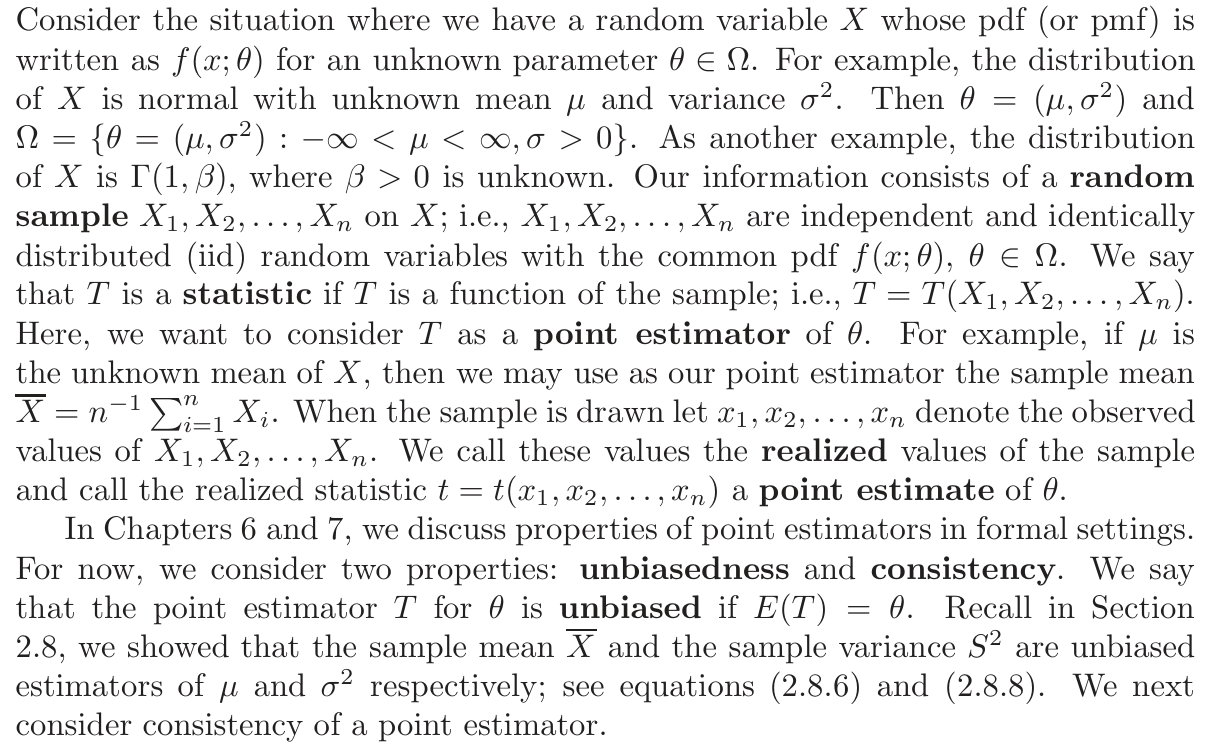
\includegraphics[width=\textwidth]{2-chap5-20250309.png}
% \caption{}
\label{}
\end{figure}

\begin{figure}[H]
\centering
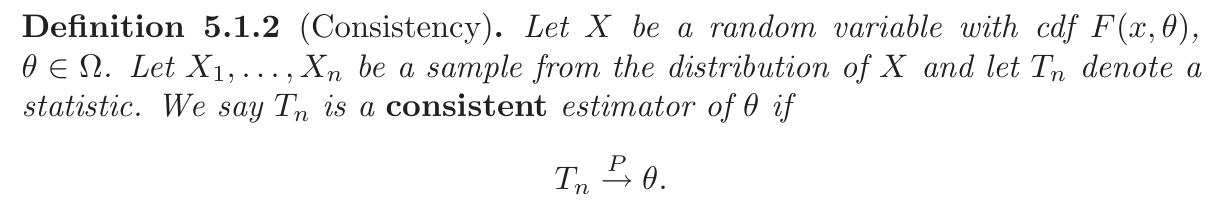
\includegraphics[width=\textwidth]{3-chap5-20250309.png}
% \caption{}
\label{}
\end{figure}

\subsection{Convergence in Distribution}

In many situations we can show statistic convergence without the distribution function of the statistic. But how close is the statistic to the estimator?

\begin{figure}[H]
\centering
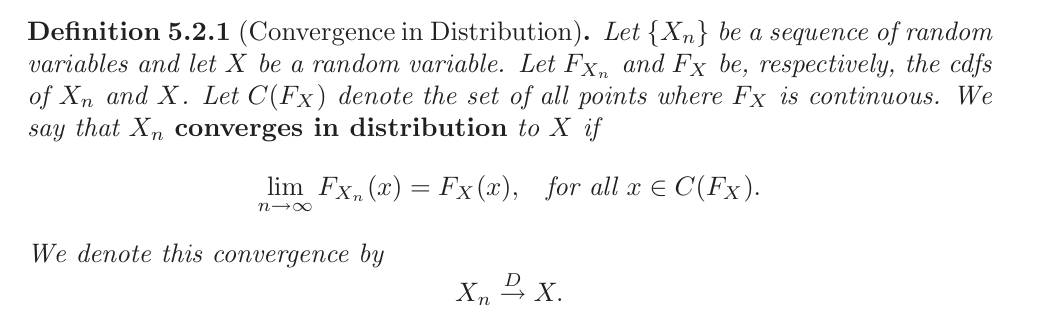
\includegraphics[width=\textwidth]{4-chap5-20250309.png}
% \caption{}
\label{}
\end{figure}

\begin{figure}[H]
\centering
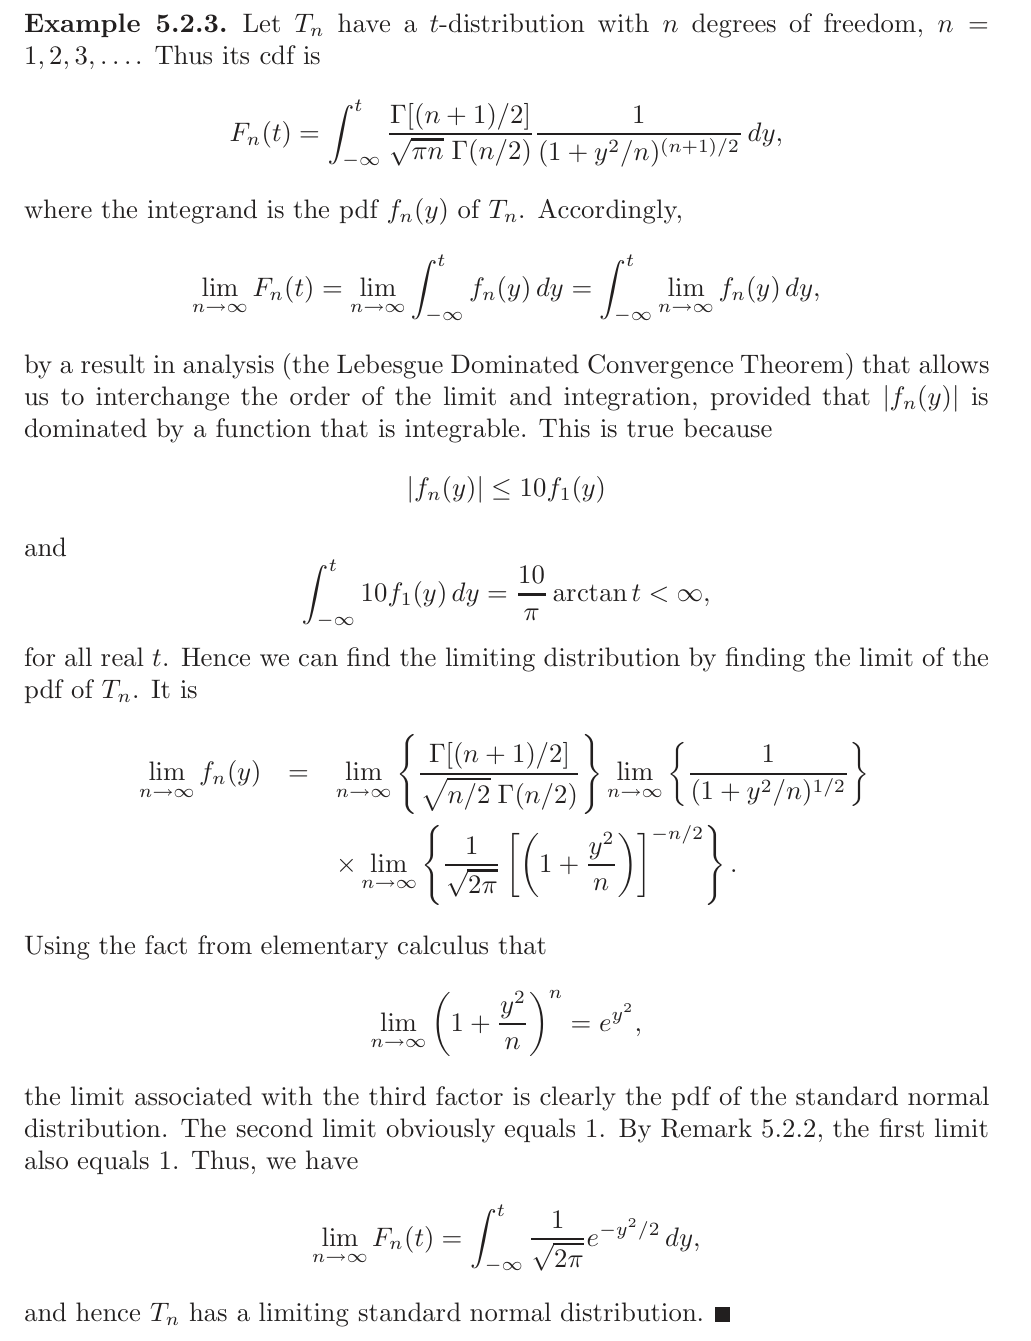
\includegraphics[width=\textwidth]{5-chap5-20250309.png}
% \caption{}
\label{}
\end{figure}

\begin{theorem}[Stirling's formula]
\[
\Gamma(k+1)\sim \sqrt{ 2\pi }k^{k+1/2 }e^{ -k }
\]
\end{theorem}
\begin{figure}[H]
\centering
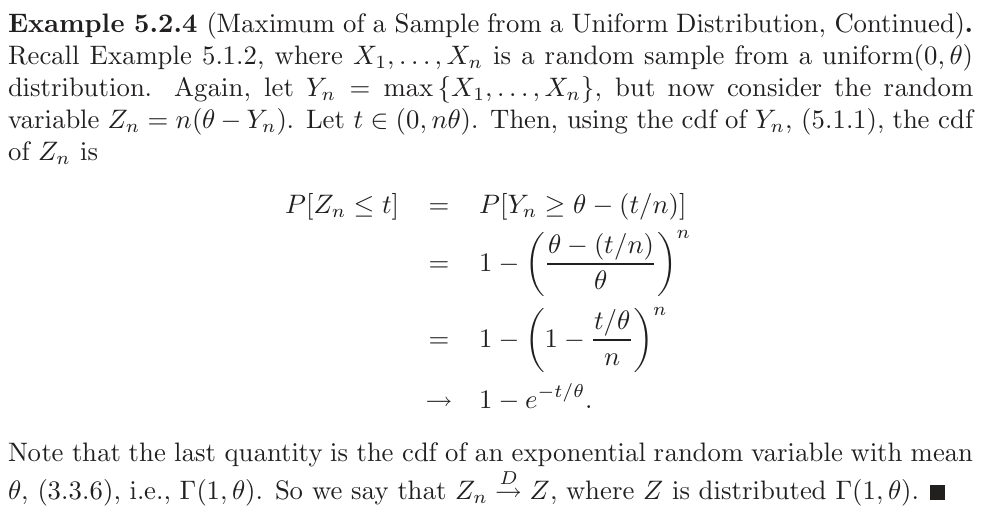
\includegraphics[width=\textwidth]{6-chap5-20250309.png}
% \caption{}
\label{}
\end{figure}

Convergence in distribution is weaker than convergence in probability. Thus convergence in distribution is often called weak convergence.

\begin{theorem}
If $X_n$ converges to $X$ in probability, then $X_n$ converges to $X$ in distribution.\label{4b6469}
\end{theorem}\begin{proof}
Let $x$ be a point of continuity of $F_{X}(x)$. For every $\epsilon>0$,
\[
\begin{aligned}
F_{X_n}(x) & =P[X_n\leq x] \\
 & =P[\{ X_n\leq x \}\cap \{ \lvert X_n-X \rvert <\epsilon \}]+P[\{ X_n\leq x \}\cap \{ \lvert X_n-X \rvert \geq \epsilon \}] \\
 & \leq P[X\leq x+\epsilon]+P[\lvert X_n-X \rvert \geq \epsilon]
\end{aligned}
\]
Basd on this inequality and the fact that $X_n\overset{ P }{ \to }X$ we see that
\[
\limsup_{ n \to \infty } F_{X_n}(x)\leq F_{X}(x+\epsilon)
\]
To get a lower bound, we proceed similarly with the complement to show that
\[
P[X_n>x]\leq P[X\geq x-\epsilon]+P[\lvert X_n-X \rvert \geq \epsilon]
\]
Hence
\[
\liminf_{ n \to \infty } F_{X_n}(x)\geq F_{X}(x-\epsilon)
\]
Using a relationship between $\limsup$ and $\liminf$, it follows that
\[
F_{X}(x-\epsilon)\leq \liminf_{ n \to \infty } F_{X_n}(x)\leq \limsup_{ n \to \infty } F_{X_n}(x)\leq F_{X}(x+\epsilon)
\]
Letting $\epsilon \downarrow0$ gives us the desired result.
\end{proof}

\begin{figure}[H]
\centering
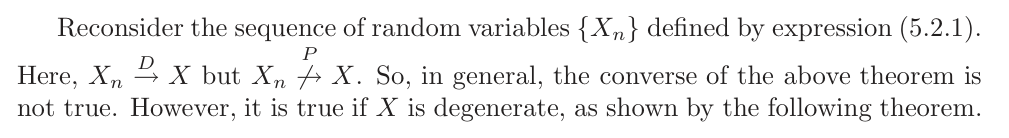
\includegraphics[width=\textwidth]{7-chap5-20250309.png}
% \caption{}
\label{}
\end{figure}

\begin{figure}[H]
\centering
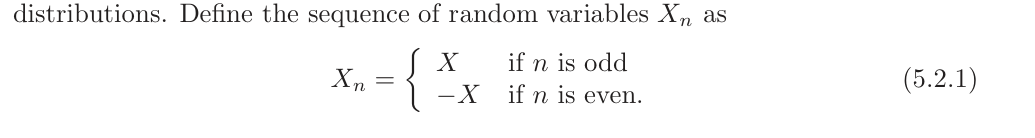
\includegraphics[width=\textwidth]{9-chap5-20250309.png}
% \caption{}
\label{}
\end{figure}

\begin{theorem}
If $X_n\overset{ D }{ \to }b$ constant, then $X_n\overset{ P }{ \to }b$.
\end{theorem}
Let $\epsilon>0$ be given. Then
\[
\lim_{ n \to \infty } P[\lvert X_n-b \rvert \leq \epsilon]=\lim_{ n \to \infty } F_{X_n}(b+\epsilon)-\lim_{ n \to \infty } F_{X_n}[(b-\epsilon)-0]=1-0=1
\]
The converse is not true.

\begin{theorem}
$X_n\overset{ D }{ \to }X,Y_n\overset{ P }{ \to }0$ then $X_n+Y_n\overset{ D }{ \to }X$.\label{e41498}
\end{theorem}

The proof is similar to the above theorem.

We often use this result as follows. Suppose it is difficult to show that $X_n$ converges to $X$ in distributino, but it is easy to show that $Y_n$ converges in distribution to $X$ and that $X_n-Y_n$ converges to 0 in probability. Hence by this last theorem. $X_n=Y_n+(X_n-Y_n)\overset{ D }{ \to }X$ as desired.

The next two theorems state general results.

\begin{theorem}
$X_n\overset{ D }{ \to }X$ and $g$ continuous on the support of $X$. Then $g(X_n)\overset{ D }{ \to }g(X)$.\label{721da5}
\end{theorem}

An often-used application of this theorem occurs when we have a sequence of random variables $Z_n$ which converges in distribution to a standard normal random variable $Z$. Because the distribution of $Z^{2}$ is $\chi^{2}(1)$, it follows by the above theorem that $Z_n^{2}$ converges in distribution to a $\chi^{2}(1)$ distribution.

\begin{theorem}[Slutsky's theorem]
If $X_n\overset{ D }{ \to }X,A_n\overset{ P }{ \to }a$ and $B_n\overset{ P }{ \to }b$ then $A_n+B_nX_n\overset{ D }{ \to }a+bX$.\label{1136a4}
\end{theorem}

The proof is similar to \cref{4b6469}

\subsection{Bounded in Probability}

\begin{figure}[H]
\centering
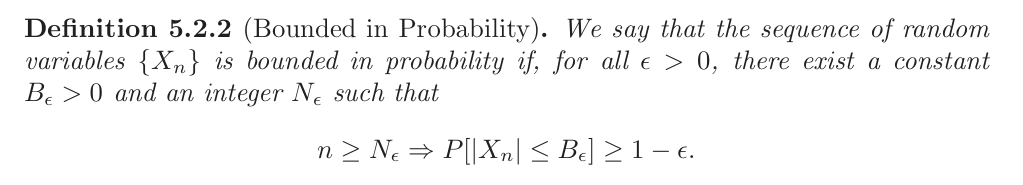
\includegraphics[width=\textwidth]{10-chap5-20250309.png}
% \caption{}
\label{}
\end{figure}

\begin{theorem}
\begin{figure}[H]
\centering
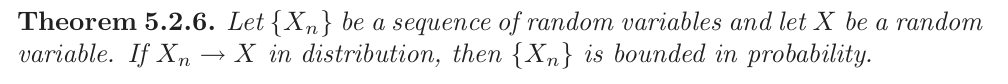
\includegraphics[width=\textwidth]{11-chap5-20250309.png}
% \caption{}
\label{}
\end{figure}\label{b809d0}
\end{theorem}

One way of thinking of a sequence that is bounded in probability (or one that is converging to a random variable in distribution) is that the probability mass of $\lvert X_n \rvert$ is not escaping to $\infty$. At times we can use boundedness in probability instead of convergence in distribution. A property we will need  later is given in the following theorem:

\begin{theorem}
Let $\{ X_n \}$ be a sequence of random variables bounded in probability and let $\{ Y_n \}$ be a sequence of random variables that converges to 0 in probability. Then
\[
X_nY_n\overset{ P }{ \to }0
\]
\end{theorem}
Let $\epsilon>0$ is given. Choose $B_{\epsilon}>0$ and an integer $N_{\epsilon}$ such that
\[
n\geq N_{\epsilon}\Rightarrow P[\lvert X_n \rvert \leq B_{\epsilon}]\geq 1-\epsilon
\]
Then
\[
\varlimsup_{ n \to \infty } P[\lvert X_nY_n \rvert \geq \epsilon]\leq \varlimsup_{ n \to \infty } P[\lvert X_nY_n \rvert \geq \epsilon,\lvert X_n \rvert \leq B_{\epsilon}]+\varlimsup_{ n \to \infty } P[\lvert X_nY_n \rvert \geq \epsilon,\lvert X_n \rvert >B_{\epsilon}]\leq \varlimsup_{ n \to \infty } P[\lvert Y_n \rvert \geq \epsilon/B_{\epsilon}]+\epsilon=\epsilon
\]
\begin{remark}
It's similar to $X_n,Y_n\overset{ P }{ \to }X,Y\Rightarrow X_nY_n\overset{ P }{ \to }XY$.
\end{remark}
\subsection{\texorpdfstring{$\Delta$}{Delta}-Method}

The $\Delta$-method is employed to determine the asymptotic distribution of a function of a random variable, given the distribution of the random variable itself. This is analogous to problems discussed in previous chapters, such as \cref{721da5} and \cref{1136a4}.

\textbf{Little-o Notation}

The notation $Y_n=o_p(X_n)$ signifies that $Y_n$ converges to 0 in probability relative to $X_n$, formally:
\[
Y_n=o_p(X_n) \text { if and only if } \frac{Y_n}{X_n} \xrightarrow{P} 0 \text {, as } n \rightarrow \infty.
\]
\textbf{Big-O Notation}

The notation $Y_n=O_p(X_n)$ indicates that $\frac{Y_n}{X_n}$ is bounded in probability as $n \rightarrow \infty$.

\begin{theorem}[Theorem 5.2.8.]
If $\{Y_n\}$ is a sequence of random variables that is bounded in probability and $X_n=o_p(Y_n)$, then $X_n \xrightarrow{P} 0$ as $n \rightarrow \infty$.\label{cf8d09}
\end{theorem}

\textbf{Proof of Theorem 5.2.8}

Let $\epsilon>0$. Then, there exist $N_{\epsilon}$ and $B_{\epsilon}$ such that for $n \geq N_{\epsilon}$, $P[|Y_n| \leq B_{\epsilon}] \geq 1-\epsilon$. Since $\frac{X_n}{Y_n} \xrightarrow{P} 0$, we have:
\[
P[|X_n| \geq \epsilon]=P[|X_n| \geq \epsilon,|Y_n| \leq B_{\epsilon}]+P[|X_n| \geq \epsilon,|Y_n| >B_{\epsilon}]\leq P\left[ \frac{X_n}{| Y_n |}\geq \frac{\epsilon}{B_{\epsilon}} \right]+P[| Y_n | >B_{\epsilon}]\to\epsilon
\]
\begin{theorem}[Theorem 5.2.9 ($\Delta$-Method)]
Let $\{X_n\}$ be a sequence of random variables such that
\[
\sqrt{n}(X_n-\theta) \xrightarrow{D} N(0, \sigma^2).
\]If $g(x)$ is differentiable at $\theta$ and $g^{\prime}(\theta) \neq 0$, then
\[
\sqrt{n}(g(X_n)-g(\theta)) \xrightarrow{D} N(0, \sigma^2(g^{\prime}(\theta))^2).
\]
\end{theorem}
\textbf{Proof of Theorem 5.2.9}

Since $g(X_n)=g(\theta)+g'(\theta)(X_n-\theta)+o_{p}(|X_n-\theta |)$, it follows that
\[
\sqrt{ n }(g(X_n)-g(\theta))=g'(\theta)\sqrt{ n }(X_n-\theta)+o_{p}(\sqrt{ n }|X_n-\theta |)
\]
Because $\sqrt{ n }(X_n-\theta)\overset{ D }{ \to }N(0,\sigma^{2})$, it implies that $\sqrt{ n }|X_n-\theta |$ is bounded in probability. Therefore, by \cref{cf8d09} , $o_{p}(\sqrt{ n }|X_n-\theta |)\to0$ in probability. Hence, the result follows.

\subsection{Moment Generating Function Technique}

It's difficult to obtain $\lim_{ n \to \infty }F_{X_n}(x)$, but quite easier from the mgf $M_n$ that corresponds to the cdf $F_{X_n}(x)$.

\begin{figure}[H]
\centering
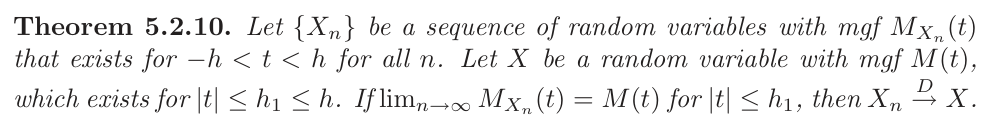
\includegraphics[width=\textwidth]{15-chap5-20250309.png}
% \caption{}
\label{}
\end{figure}

\begin{figure}[H]
\centering
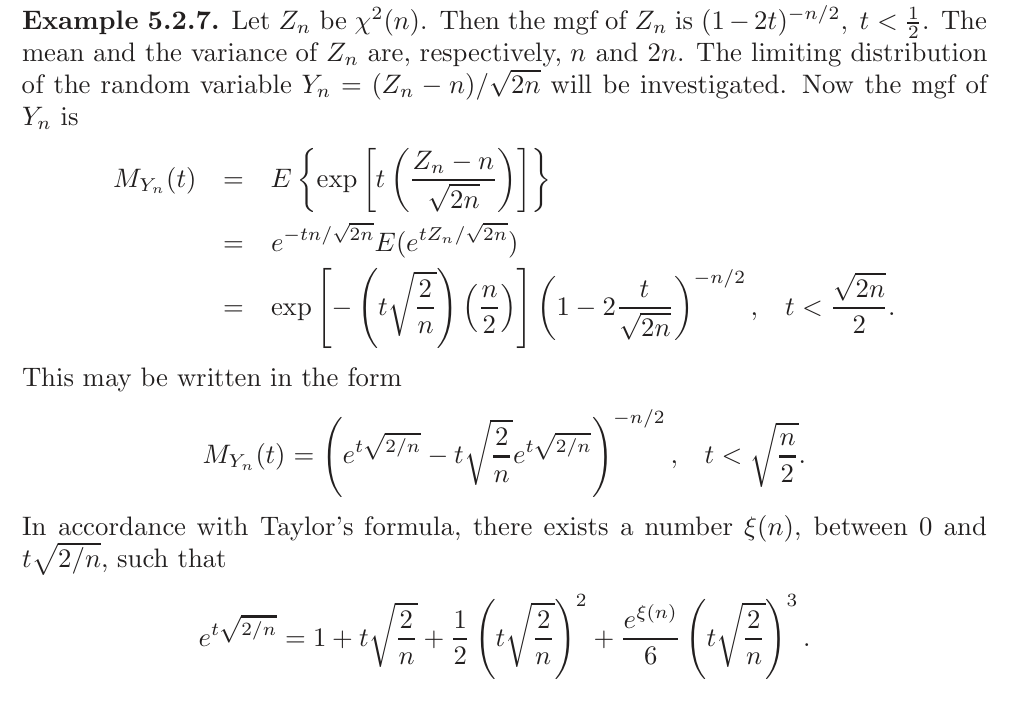
\includegraphics[width=\textwidth]{16-chap5-20250309.png}
% \caption{}
\label{}
\end{figure}

\begin{figure}[H]
\centering
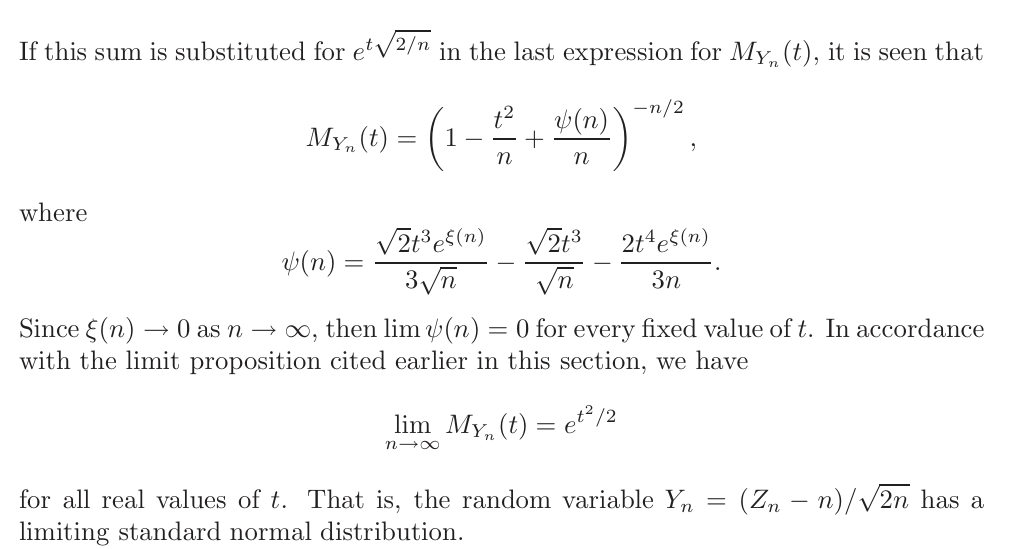
\includegraphics[width=\textwidth]{17-chap5-20250309.png}
% \caption{}
\label{}
\end{figure}

\subsection{Central Limit Theorem}

\begin{figure}[H]
\centering
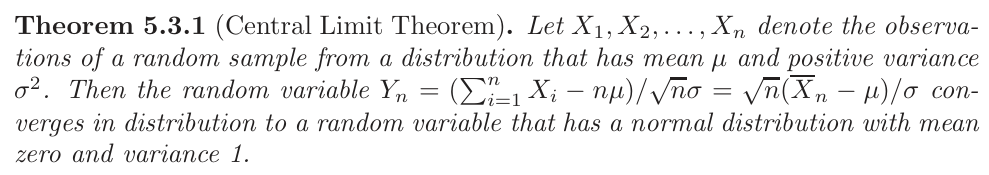
\includegraphics[width=\textwidth]{18-chap5-20250309.png}
% \caption{}
\label{}
\end{figure}

Prove by characteristic function $\varphi(t)=E(e^{ itX })$.

The Central Limit Theorem is saying that when $n$ is large, fixed positive integer, the random variable $\overline{X}$ has an approximate normal distribution with mean $\mu$ and variance $\sigma^{2}/n$. We can equivalently state the conclusion of the Central Limit Theorem as
\[
\sqrt{ n }(\overline{X}-\mu)\overset{ \mathcal{D} }{ \to }N(0,\sigma^{2})
\]
This is often a convenient formulation to use.

\begin{remark}
We know that $\overline{X}$ and $\sum_{i=1}^{n}X_i$ have approximately normal distributions, provided that $n$ is large enough. Later, we find that other statistics also have approximate normal distributions, and this is the reason that the normal distribution is so improtant to statisticians. That is, while not many underlying distributions are normal, the distributions of statistics calculated from random samples arising from these distributions are often close to being normal.
\end{remark}
We can combine $\Delta$ -method with Central Limit Theorem. Assume that $X_1,\dots,X_n$ is a random sample on $X$ which has finite mean $\mu$ and variance $\sigma^{2}$. Then by the Central Limit Theorem, we have
\[
\sqrt{ n }(\overline{X}-\mu)\overset{ \mathcal{D} }{ \to }N(0,\sigma^{2})
\]
Hence by the $\Delta$ -method, we have
\[
\sqrt{ n }[g(\overline{X})-g(\mu)]\overset{ \mathcal{D} }{ \to }N(0,\sigma^{2}(g'(\mu))^{2})
\]
for a continuous transformation $g(x)$ such that $g'(\mu)\neq0$.

\subsection{Extensions to Multivariate Distributions}

This section discusses asymptotic concepts for sequences of random vectors.

\begin{definition}[convergence in probability]
Let $\{\mathbf{X}_n\}$ be a sequence of $p$-dimensional random vectors, and let $\mathbf{X}$ be a random vector, all defined on the same sample space. We say that $\{\mathbf{X}_n\}$ \textbf{converges in probability} to $\mathbf{X}$ if
\[
\lim_{n \rightarrow \infty} P\left[\left\|\mathbf{X}_n-\mathbf{X}\right\| \geq \epsilon\right]=0
\]for all $\epsilon>0$. As in the univariate case, we write $\mathbf{X}_n \xrightarrow{P} \mathbf{X}$.
\end{definition}
\begin{theorem}[Theorem 5.4.1]
Let $\{\mathbf{X}_n\}$ be a sequence of $p$-dimensional random vectors, and let $\mathbf{X}$ be a random vector, all defined on the same sample space. Then $\mathbf{X}_n \xrightarrow{P} \mathbf{X}$ if and only if $X_{n j} \xrightarrow{P} X_j$ for all $j=1, \ldots, p$.\label{479de5}
\end{theorem}

Based on \cref{479de5}, many theorems involving convergence in probability can be extended to the multivariate setting.

Let $\{ \mathbf{X}_n \}$ be a sequence of i.i.d. random vectors with common mean vector $\boldsymbol{\mu}$ and variance-covariance matrix $\boldsymbol{\Sigma}$. Denote the vector of means by $\mathbf{\overline{X}}_n=\frac{1}{n}\sum_{i=1}^{n}\mathbf{X}_i$. By the Weak Law of Large Numbers, $\overline{X}_j\to \mu _j$ in probability for each $j$. Hence, by \cref{479de5}, $\overline{\mathbf{X}}_n\to \boldsymbol{\mu}$ in probability.

Now consider the analog of the sample variances. Let $\mathbf{X}_i=(X_{i1},\dots,X_{ip})'$. Define the sample variances and covariances by
\[
S_{n,jj}=S_{n,j}^{2}=\frac{1}{n-1}\sum_{i=1}^{n} (X_{ij}-\overline{X}_j)^{2}\quad \text{for }j=1,\dots,p
\]
\[
S_{n,jk}=\frac{1}{n-1}\sum_{i=1}^{n} (X_{ij}-\overline{X}_j)(X_{ik}-\overline{X}_k)\quad \text{for }j\neq k=1,\dots,p
\]
If we define the $p\times p$ matrix $\mathbf{S}=(S_{n,jk})$, then $\mathbf{S}\to\boldsymbol{\Sigma}$ in probability.

\begin{definition}[convergence in distribution]
Let $\{\mathbf{X}_n\}$ be a sequence of random vectors with $\mathbf{X}_n$ having distribution function $F_n(\mathbf{x})$, and let $\mathbf{X}$ be a random vector with distribution function $F(\mathbf{x})$. Then $\{\mathbf{X}_n\}$ \textbf{converges in distribution} to $\mathbf{X}$ if
\[
\lim_{n\rightarrow \infty}F_n(\mathbf{x})=F(\mathbf{x}),
\]for all points $\mathbf{x}$ at which $F(\mathbf{x})$ is continuous. We write $\mathbf{X}_n \xrightarrow{D} \mathbf{X}$.
\end{definition}
\begin{theorem}
Let $\{\mathbf{X}_n\}$ be a sequence of random vectors that converges in distribution to a random vector $\mathbf{X}$, and let $g(\mathbf{x})$ be a function that is continuous on the support of $\mathbf{X}$. Then $g(\mathbf{X}_n)$ converges in distribution to $g(\mathbf{X})$.
\end{theorem}
\begin{theorem}
Let $\{\mathbf{X}_n\}$ be a sequence of random vectors with $\mathbf{X}_n$ having distribution function $F_n(\mathbf{x})$ and moment generating function $M_n(\mathbf{t})$. Let $\mathbf{X}$ be a random vector with distribution function $F(\mathbf{x})$ and moment generating function $M(\mathbf{t})$. Then $\{\mathbf{X}_n\}$ converges in distribution to $\mathbf{X}$ if and only if, for some $h>0$,
\[
\lim_{n\rightarrow \infty}M_n(\mathbf{t})=M(\mathbf{t}),
\]for all $\mathbf{t}$ such that $\|\mathbf{t}\|<h$.
\end{theorem}
\begin{theorem}[Multivariate Central Limit Theorem]
Let $\{\mathbf{X}_n\}$ be a sequence of i.i.d. random vectors with common mean vector $\boldsymbol{\mu}$ and variance-covariance matrix $\boldsymbol{\Sigma}$ which is positive definite. Assume that the common moment generating function $M(\mathbf{t})$ exists in an open neighborhood of $\mathbf{0}$. Let
\[
\mathbf{Y}_n=\frac{1}{\sqrt{n}} \sum_{i=1}^n\left(\mathbf{X}_i-\boldsymbol{\mu}\right)=\sqrt{n}(\overline{\mathbf{X}}-\boldsymbol{\mu})
\]Then $\mathbf{Y}_n$ converges in distribution to a $N_p(\mathbf{0}, \boldsymbol{\Sigma})$ distribution.
\end{theorem}
\textbackslash{}begin\{proof\}
Let $\mathbf{t}\in \mathbf{R}^{p}$ be a vector in the stipulated neighborhood of $\mathbf{0}$. The moment generating function of $\mathbf{Y}_n$ is
\[
M_n(\mathbf{t})=\mathbb{E}\left[ \exp \left\{  \mathbf{t}'\frac{1}{\sqrt{ n }} \sum_{i=1}^{n} (\mathbf{X}_i-\boldsymbol{\mu})  \right\} \right]=\mathbb{E}\left[ \exp \left\{  \frac{1}{\sqrt{ n }} \sum_{i=1}^{n} \mathbf{t}'(\mathbf{X}_i-\boldsymbol{\mu})  \right\} \right]=\mathbb{E}\left[ \exp \left\{  \frac{1}{\sqrt{ n }} \sum_{i=1}^{n} W_i  \right\} \right]
\]
where $W_i=\mathbf{t}'(\mathbf{X}_i-\boldsymbol{\mu})$. Note that $W_i$ are i.i.d. with mean 0 and variance $\mathrm{Var}(W_i)=\mathbf{t}'\boldsymbol{\Sigma}\mathbf{t}$. Hence, by the standard Central Limit Theorem,
\[
\frac{1}{\sqrt{ n }}\sum_{i=1}^{n} W_i\overset{ D }{ \to }N(0,\mathbf{t}'\boldsymbol{\Sigma}\mathbf{t})
\]
Then $M_n(\mathbf{t})$ is the MGF of $(1/\sqrt{ n })\sum_{i=1}^{n}W_i$ evaluated at 1. Therefore, we must have
\[
M_n(\mathbf{t})=\mathbb{E}\left[ \exp \left\{  1\cdot \frac{1}{\sqrt{ n }} \sum_{i=1}^{n} W_i  \right\} \right]\to e^{ 1^{2}\mathbf{t}'\boldsymbol{\Sigma}\mathbf{t}/2 }=e^{ \mathbf{t}'\boldsymbol{\Sigma}\mathbf{t}/2 }.
\]
Because the last quantity is the moment generating function of a $N_{p}(\mathbf{0},\boldsymbol{\Sigma})$ distribution, the result follows.
\textbackslash{}end\{proof\}

\begin{theorem}[Theorem 5.4.5]
Let $\{\mathbf{X}_n\}$ be a sequence of $p$-dimensional random vectors. Suppose $\mathbf{X}_n \xrightarrow{D} N(\boldsymbol{\mu}, \boldsymbol{\Sigma})$. Let $\mathbf{A}$ be an $m \times p$ matrix of constants, and let $\mathbf{b}$ be an $m$-dimensional vector of constants. Then $\mathbf{A} \mathbf{X}_n+\mathbf{b} \xrightarrow{D} N\left(\mathbf{A} \boldsymbol{\mu}+\mathbf{b}, \mathbf{A} \boldsymbol{\Sigma} \mathbf{A}^{\prime}\right)$.
\end{theorem}
\begin{theorem}[Theorem 5.4.6]
Let $\{\mathbf{X}_n\}$ be a sequence of $p$-dimensional random vectors. Suppose
\[
\sqrt{n}\left(\mathbf{X}_n-\boldsymbol{\mu}_0\right) \xrightarrow{D} N_p(\mathbf{0}, \boldsymbol{\Sigma}) .
\]Let $\mathbf{g}$ be a transformation $\mathbf{g}(\mathbf{x})=\left(g_1(\mathbf{x}), \ldots, g_k(\mathbf{x})\right)^{\prime}$ such that $1 \leq k \leq p$ and the $k \times p$ matrix of partial derivatives,
\[
\mathbf{B}=\left[\frac{\partial g_i}{\partial \mu_j}\right], \quad i=1, \ldots k ; j=1, \ldots, p
\]are continuous and do not vanish in a neighborhood of $\boldsymbol{\mu}_0$. Let $\mathbf{B}_0=\mathbf{B}$ at $\boldsymbol{\mu}_0$. Then
\[
\sqrt{n}\left(\mathbf{g}\left(\mathbf{X}_n\right)-\mathbf{g}\left(\boldsymbol{\mu}_0\right)\right) \xrightarrow{D} N_k\left(\mathbf{0}, \mathbf{B}_0 \boldsymbol{\Sigma} \mathbf{B}_0^{\prime}\right) .
\]
\end{theorem}